\documentclass[11pt]{article}

\usepackage[margin=1in]{geometry}
\usepackage[T1]{fontenc}
\usepackage{lmodern}
\usepackage{microtype}
\usepackage{amsmath,amssymb,amsthm,mathtools}
\usepackage[dvipsnames]{xcolor}
\usepackage[most]{tcolorbox}
\usepackage{tikz}
\usetikzlibrary{decorations.markings}
\usepackage{enumitem}
\usepackage{tocloft}
\usepackage[hidelinks]{hyperref}

\definecolor{courseblue}{HTML}{1F4E79}
\definecolor{lightblue}{HTML}{EAF2F8}
\definecolor{lightgreen}{HTML}{EAF7EA}
\definecolor{lightpink}{HTML}{FCE8EF}
\definecolor{lightyellow}{HTML}{FFF8D6}
\definecolor{warningyellow}{HTML}{D6A000}
\definecolor{exercisebg}{HTML}{D6E6F5}
\definecolor{exerciseframe}{HTML}{1F4E79}
\definecolor{examplebg}{HTML}{F4FAFE}
\definecolor{exampleframe}{HTML}{85C1E9}
\definecolor{darkgray}{HTML}{333333}
\definecolor{lightorange}{HTML}{FDEBD8}
\definecolor{orangeframe}{HTML}{E08A3C}

\setlength{\parindent}{0pt}
\setlength{\parskip}{0.65em}
\setlist[itemize]{topsep=0.25em,itemsep=0.15em}
\renewcommand{\cftsecleader}{\cftdotfill{\cftdotsep}}
\renewcommand{\cftsubsecleader}{\cftdotfill{\cftdotsep}}

\theoremstyle{plain}
\newtheorem{theorem}{Theorem}[section]
\newtheorem{proposition}[theorem]{Proposition}
\newtheorem{lemma}[theorem]{Lemma}
\newtheorem{corollary}[theorem]{Corollary}
\theoremstyle{definition}
\newtheorem{definition}[theorem]{Definition}
\newtheorem{example}[theorem]{Example}
\newtheorem{exercise}[theorem]{Exercise}
\theoremstyle{remark}
\newtheorem*{remark}{Remark}
\newtheorem*{fact}{Fact}
\newtheorem*{warning}{Warning}

\tcolorboxenvironment{definition}{
  enhanced,
  unbreakable,
  colback=lightgreen,
  colframe=ForestGreen,
  boxrule=0.7pt,
  arc=2pt,
  left=6pt,
  right=6pt,
  top=5pt,
  bottom=5pt
}

\tcolorboxenvironment{warning}{
  enhanced,
  colback=lightyellow,
  colframe=warningyellow,
  boxrule=0.7pt,
  arc=2pt,
  left=6pt,
  right=6pt,
  top=5pt,
  bottom=5pt
}

\tcolorboxenvironment{exercise}{
  enhanced,
  colback=exercisebg,
  colframe=exerciseframe,
  boxrule=1pt,
  arc=2pt,
  left=6pt,
  right=6pt,
  top=5pt,
  bottom=5pt
}

\tcolorboxenvironment{example}{
  enhanced,
  colback=examplebg,
  colframe=exampleframe,
  boxrule=0.7pt,
  arc=2pt,
  left=6pt,
  right=6pt,
  top=5pt,
  bottom=5pt
}

\numberwithin{equation}{section}

\newcommand{\be}{\begin{eqnarray}}
\newcommand{\ee}{\end{eqnarray}}
\newcommand{\C}{\mathbb{C}}
\newcommand{\R}{\mathbb{R}}
\newcommand{\N}{\mathbb{N}}

\DeclareMathOperator{\Hol}{\mathcal{H}\mathrm{ol}}
\DeclareMathOperator{\Real}{Re}
\DeclareMathOperator{\Imag}{Im}
\newcommand{\A}{\mathcal{A}}
\newcommand{\CT}{\C[[T]]}
\newcommand{\CLT}{\C((T))}
\tcbset{breakable}
\begin{document}

\begin{center}
  \colorbox{lightblue}{%
    \begin{minipage}{0.94\textwidth}
      \vspace{0.55em}
      \begin{tabular*}{\textwidth}{@{\extracolsep{\fill}}lr}
        {\color{courseblue}\bfseries\LARGE Lecture 13} &
        {\color{courseblue}\bfseries\LARGE MATH 411}\\[0.35em]
        \textbf{Fall 2026} & \textbf{Date: Oct 5, 2026}\\
        & \textbf{Instructor: Manish Patnaik}
      \end{tabular*}
      \vspace{0.45em}
    \end{minipage}}
\end{center}

\setcounter{tocdepth}{1}
\tableofcontents
\vspace{0.45em}

% Handwritten page 1.
\section{Where we are}
\noindent
\begin{minipage}[c]{0.6\textwidth}
Last time we proved Goursat's theorem: if $f$ is holomorphic on an open set
$U$ and $R\subseteq U$ is a rectangle, then
\be
 \int_{\partial R}f=0.
\ee
\end{minipage}\hfill
\begin{minipage}[c]{0.36\textwidth}
\centering
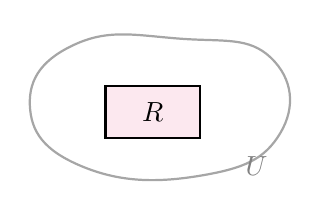
\begin{tikzpicture}[scale=0.6]
  \draw[thick,gray!70] plot[smooth cycle,tension=0.8]
    coordinates {(-2.6,0.2) (-1.6,1.5) (0.6,1.6) (2.5,1.2) (2.7,-0.4) (1.0,-1.3) (-1.5,-1.1)};
  \draw[thick,fill=lightpink] (-1,-0.5) rectangle (1,0.6);
  \node at (0,0.05) {$R$};
  \node[gray] at (2.2,-1.1) {$U$};
\end{tikzpicture}
\end{minipage}

This has many consequences:
\begin{itemize}
  \item \emph{theoretical}: existence of primitives, Cauchy's theorem on a
  disc (today);
  \item \emph{practical}: computation of \emph{real} integrals, such as
  \be
   \int_0^\infty\frac{1-\cos x}{x^2}\,dx=\frac\pi2
  \ee
  (next time).
\end{itemize}

\section{Primitives}
\begin{definition}[Primitive]
Let $f$ be a continuous function on an open set $U\subseteq\C$. A
\emph{primitive} for $f$ (or \emph{holomorphic primitive}) is a function
$g\colon U\to\C$ such that $g$ is holomorphic and
\be
 g'=f\qquad\text{on }U.
\ee
\end{definition}

% Handwritten page 2.
\begin{example}[Analytic functions have local primitives]
\label{ex:local-prim}
Recall: if $f$ is analytic on $U$, so
\be
 f(z)=\sum a_n(z-z_0)^n\qquad\text{for $z$ near $z_0$},
\ee
then $f'(z)$ exists and is computed term by term. But we can also
``integrate term by term'' to get the series
\be
 g(z)=\sum_n\frac{a_n}{n+1}(z-z_0)^{n+1}.
\ee
What do we know about this series? Its coefficient of $(z-z_0)^{n+1}$ is
$\frac{a_n}{n+1}$, and
\be
 \limsup_n\left|\frac{a_n}{n+1}\right|^{1/n}
 =\limsup_n\frac{|a_n|^{1/n}}{(n+1)^{1/n}}
 =\limsup_n|a_n|^{1/n},
\ee
since $(n+1)^{1/n}\to1$. (Shifting the index by one does not change the
radius of convergence.) Therefore $g(z)$ is also convergent for $z$ near
$z_0$, so
\be
 g(z)\ \text{analytic}\ \Longrightarrow\ \text{holomorphic, and}\ g'=f
\ee
by term-by-term differentiation. So $g$ is a primitive for $f$ on a disc
around $z_0$.
\end{example}

\subsection*{Some remarks on primitives}
\begin{proposition}
\label{prop:prim-eval}
If you have a primitive for $f$, then path integrals are easy to compute. Let
$f$ be continuous on $U$ with primitive $g$, and $\gamma\colon[a,b]\to U$ a
path. Then
\be
 \int_\gamma f=g\bigl(\gamma(b)\bigr)-g\bigl(\gamma(a)\bigr).
\ee
\end{proposition}

\noindent
\begin{minipage}[c]{0.36\textwidth}
\centering
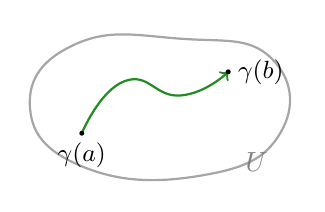
\begin{tikzpicture}[scale=0.6]
  \draw[thick,gray!70] plot[smooth cycle,tension=0.8]
    coordinates {(-2.6,0.2) (-1.6,1.5) (0.6,1.6) (2.5,1.2) (2.7,-0.4) (1.0,-1.3) (-1.5,-1.1)};
  \draw[ForestGreen,thick,->] plot[smooth,tension=0.9] coordinates {(-1.5,-0.4) (-0.6,0.7) (0.6,0.4) (1.6,0.9)};
  \fill (-1.5,-0.4) circle (1.5pt) node[below,font=\small]{$\gamma(a)$};
  \fill (1.6,0.9) circle (1.5pt) node[right,font=\small]{$\gamma(b)$};
  \node[gray] at (2.2,-1.0) {$U$};
\end{tikzpicture}
\end{minipage}\hfill
\begin{minipage}[c]{0.6\textwidth}
\begin{proof}
% Handwritten page 3.
Since $g'=f$ ($g$ is a primitive for $f$), the chain rule gives
\be
 \frac{d}{dt}\,g\bigl(\gamma(t)\bigr)=g'\bigl(\gamma(t)\bigr)\,\gamma'(t)
 =f\bigl(\gamma(t)\bigr)\,\gamma'(t).
\ee
Therefore, by FTC,
\be
 \int_\gamma f=\int_a^b\frac{d}{dt}\,g\bigl(\gamma(t)\bigr)\,dt
 =g\bigl(\gamma(b)\bigr)-g\bigl(\gamma(a)\bigr). \qedhere
\ee
\end{proof}
\end{minipage}

So the answer is computed in terms of the primitive and the endpoints of the
curve $\gamma$.

\begin{exercise}
Justify the chain rule used above: if $g$ is holomorphic and $\gamma$ is
differentiable at $t$, then $\frac{d}{dt}g(\gamma(t))=g'(\gamma(t))\gamma'(t)$.
\emph{Hint.} Write $g(w)-g(w_0)=\bigl(g'(w_0)+\varphi(w)\bigr)(w-w_0)$ with
$\varphi(w)\to0$ as $w\to w_0$, and take $w=\gamma(t+s)$, $w_0=\gamma(t)$.
\end{exercise}

\begin{corollary}
\label{cor:closed-zero}
If $f$ admits a primitive on $U$ and $\gamma$ is a closed path in $U$
($\gamma(a)=\gamma(b)$), then $\int_\gamma f=0$.
\end{corollary}

\begin{warning}
Suppose $f$ is analytic on $U$ and $\gamma$ is a closed path in $U$. Is
$\int_\gamma f=0$? Example~\ref{ex:local-prim} only gives a primitive
\emph{near each point}, not necessarily one on all of $U$. Indeed, for
$f(z)=\frac1z$ on $U=\C\setminus\{0\}$ and $\gamma$ the unit circle, we
computed $\int_\gamma f=2\pi i\neq0$ in Lecture~11. So $\frac1z$ has no
primitive on $\C\setminus\{0\}$, even though it is analytic there.
\end{warning}

\begin{proposition}
\label{prop:closed-prim}
Let $U\subseteq\C$ be open and connected, and $f\colon U\to\C$ continuous.
If $\int_\gamma f=0$ for all closed paths $\gamma$ in $U$, then $f$ has a
primitive.
\end{proposition}

% Handwritten page 4.
Why? We need to construct a holomorphic primitive to $f$.

\noindent
\begin{minipage}[c]{0.4\textwidth}
\centering
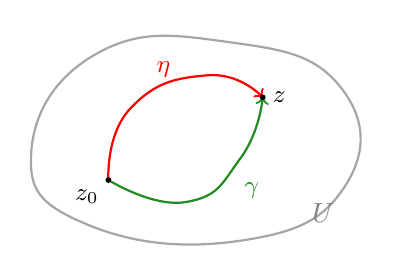
\begin{tikzpicture}[scale=0.7]
  \draw[thick,gray!70] plot[smooth cycle,tension=0.8]
    coordinates {(-2.8,0.0) (-1.6,1.8) (0.8,2.0) (2.8,1.2) (2.9,-0.6) (1.0,-1.6) (-1.8,-1.3)};
  \coordinate (a) at (-1.4,-0.5); \coordinate (b) at (1.4,1.0);
  \draw[red,thick,->] plot[smooth,tension=0.9] coordinates {(-1.4,-0.5) (-1.0,0.8) (0.4,1.4) (1.4,1.0)};
  \draw[ForestGreen,thick,->] plot[smooth,tension=0.9] coordinates {(-1.4,-0.5) (0.0,-0.9) (1.0,-0.1) (1.4,1.0)};
  \fill (a) circle (1.5pt) node[below left,font=\small]{$z_0$};
  \fill (b) circle (1.5pt) node[right,font=\small]{$z$};
  \node[red,font=\small] at (-0.4,1.5) {$\eta$};
  \node[ForestGreen,font=\small] at (1.2,-0.7) {$\gamma$};
  \node[gray] at (2.5,-1.1) {$U$};
\end{tikzpicture}
\end{minipage}\hfill
\begin{minipage}[c]{0.56\textwidth}
\emph{Idea.} Fix $z_0\in U$. For $z\in U$, choose any path $\gamma$
connecting $z_0$ and $z$ (possible since $U$ is connected), and set
\be
 g(z)=\int_\gamma f.
\ee
\end{minipage}

Why is this a well-defined function, i.e.\ independent of the path
$\gamma$? If $\eta$ is another path from $z_0$ to $z$, then $\gamma+\eta^-$
(go along $\gamma$, then back along $\eta$ reversed) is a closed loop, so
\be
 0=\int_{\gamma+\eta^-}f=\int_\gamma f+\int_{\eta^-}f=\int_\gamma f-\int_\eta f,
 \qquad\therefore\quad\int_\gamma f=\int_\eta f.
\ee
So $g$ is well-defined. But is it holomorphic with $g'=f$? We will prove a
similar statement below; the same argument works here (Exercise).

% Handwritten page 5.
\section{Primitives on a disc}
\begin{theorem}
\label{thm:disc-prim}
Let $U$ be an open disc centred at $z_0\in\C$, and $f$ a continuous function
on $U$. Assume
\be
 \int_{\partial R}f=0\qquad\text{for any rectangle }R\subseteq U.
\ee
For $z_1\in U$ define
\be
 g(z_1)=\int_{z_0}^{z_1}f,
\ee
where we choose any rectangular path connecting $z_0$ and $z_1$ (i.e.\ one
horizontal and one vertical segment). Then $g$ is a well-defined
holomorphic primitive for $f$.
\end{theorem}

\begin{center}
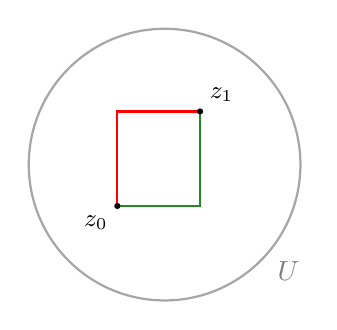
\begin{tikzpicture}[scale=0.75]
  \draw[thick,gray!70] (0,0) circle (2.3);
  \coordinate (z0) at (-0.8,-0.7); \coordinate (z1) at (0.6,0.9);
  \draw[ForestGreen,thick] (-0.8,-0.7) -- (0.6,-0.7) -- (0.6,0.9);
  \draw[red,thick] (-0.8,-0.7) -- (-0.8,0.9) -- (0.6,0.9);
  \fill (z0) circle (1.5pt) node[below left,font=\small]{$z_0$};
  \fill (z1) circle (1.5pt) node[above right,font=\small]{$z_1$};
  \node[gray] at (2.1,-1.8) {$U$};
\end{tikzpicture}
\end{center}

Note that the rectangle with opposite corners $z_0$ and $z_1$ lies in $U$:
its farthest point from the centre $z_0$ is $z_1$. So both rectangular
paths lie in $U$.

\begin{corollary}[Cauchy's theorem on a disc]
\label{cor:cauchy-disc}
If $f$ is holomorphic on a disc $U$, then
\be
 \int_\gamma f=0\qquad\text{for any closed path $\gamma$ in $U$.}
\ee
\end{corollary}

\begin{proof}
By Goursat's theorem, $\int_{\partial R}f=0$ for every rectangle
$R\subseteq U$; and $f$ is continuous since it is holomorphic. By
Theorem~\ref{thm:disc-prim}, $f$ has a primitive on $U$, so
$\int_\gamma f=0$ by Corollary~\ref{cor:closed-zero}.
\end{proof}

\begin{proof}[Proof of Theorem~\ref{thm:disc-prim}]
\textbf{1) Well-definedness.} Same idea as in
Proposition~\ref{prop:closed-prim}: the two rectangular paths from $z_0$ to
$z_1$ (horizontal-then-vertical, and vertical-then-horizontal) together form
$\pm\partial R$, where $R$ is the rectangle with opposite corners $z_0,z_1$.
Since $\int_{\partial R}f=0$, the two paths give the same integral. (If
$z_0$ and $z_1$ share a real or imaginary part, there is only one such path.)
From now on we compute $g$ using the horizontal-then-vertical path.

% Handwritten page 6.
\textbf{2) $g$ is holomorphic and $g'=f$.} Given $z_1\in U$, we want to show
\be
 \lim_{h\to0}\frac{g(z_1+h)-g(z_1)}{h}=f(z_1).
\ee

\noindent
\begin{minipage}[c]{0.44\textwidth}
\centering
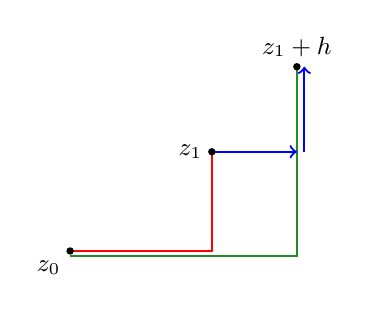
\begin{tikzpicture}[scale=0.9]
  \coordinate (z0) at (0,0);
  \coordinate (b) at (2,0); \coordinate (z1) at (2,1.4);
  \coordinate (a) at (3.2,0); \coordinate (c) at (3.2,1.4); \coordinate (zh) at (3.2,2.6);
  \draw[red,thick] (z0) -- (b) -- (z1);
  \draw[ForestGreen,thick] ([yshift=-2pt]z0) -- ([yshift=-2pt]a) -- (zh);
  \draw[blue,thick,->] (z1) -- (c);
  \draw[blue,thick,->] ([xshift=3pt]c) -- ([xshift=3pt]zh);
  \fill (z0) circle (1.5pt) node[below left,font=\small]{$z_0$};
  \fill (z1) circle (1.5pt) node[left,font=\small]{$z_1$};
  \fill (zh) circle (1.5pt) node[above,font=\small]{$z_1+h$};
\end{tikzpicture}
\end{minipage}\hfill
\begin{minipage}[c]{0.52\textwidth}
We claim that $g(z_1+h)-g(z_1)$ is the integral of $f$ over the
\textcolor{blue}{blue} path from $z_1$: horizontally, then vertically to $z_1+h$.
\end{minipage}

\be
 g(z_1+h)-g(z_1)=\int_{\text{\textcolor{ForestGreen}{green}}}f-\int_{\text{\textcolor{red}{red}}}f=\int_{z_1}^{z_1+h}f.
\ee

Indeed, the green path minus the red path minus the blue path is (up to
sign) the boundary of the rectangle with corners $\Real z_1+i\Imag z_0$,
$\Real(z_1+h)+i\Imag z_0$, $\Real(z_1+h)+i\Imag z_1$ and $z_1$. For $h$
small this rectangle lies in the disc $U$ (all four corners do, and a disc is
convex), so its boundary integral vanishes by hypothesis.

Now
\be
 \frac{g(z_1+h)-g(z_1)}{h}=\frac1h\int_{z_1}^{z_1+h}f(z)\,dz
 \qquad\text{(over the blue path).}
\ee
Since $f$ is continuous, there is $\psi(z)$ with
\be
 f(z)=f(z_1)+\psi(z)\qquad\text{and}\qquad\lim_{z\to z_1}\psi(z)=0.
\ee
Plugging this in,
\be
 \frac{g(z_1+h)-g(z_1)}{h}
 =\frac1h\left[\int_{z_1}^{z_1+h}f(z_1)\,dz+\int_{z_1}^{z_1+h}\psi(z)\,dz\right].
\ee

% Handwritten page 7.
The constant $f(z_1)$ has primitive $f(z_1)\,z$, so by
Proposition~\ref{prop:prim-eval}
\be
 \frac1h\int_{z_1}^{z_1+h}f(z_1)\,dz=\frac1h\,f(z_1)\bigl((z_1+h)-z_1\bigr)=f(z_1).
\ee
For the second term, by the ML-estimate,
\be
 \left|\frac1h\int_{z_1}^{z_1+h}\psi(z)\,dz\right|
 \leq\max_{\text{blue}}|\psi(z)|\cdot\frac1{|h|}\cdot\operatorname{arclength}(\text{blue})
 \leq2\max_{\text{blue}}|\psi(z)|,
\ee
since the blue path has length $|\Real h|+|\Imag h|\leq2|h|$. As $h\to0$, the
blue path shrinks to $z_1$, so $\max_{\text{blue}}|\psi|\to0$. Therefore
\be
 \lim_{h\to0}\frac{g(z_1+h)-g(z_1)}{h}=f(z_1),
\ee
i.e.\ $g$ is holomorphic on $U$ with $g'=f$.
\end{proof}

\end{document}
